\documentclass[12pt]{article}

% add some essential packages, some might not be used
%\usepackage{CJKutf8}
\usepackage[T1]{fontenc}
\usepackage[utf8]{inputenc}
\usepackage[usenames,dvipsnames]{color}
\usepackage{authblk}
\usepackage{xeCJK}
\usepackage{ragged2e}
\usepackage{amsmath}
%\usepackage[a4paper,margin=2in,bottom=1.0in]{geometry}
\usepackage{url}
\usepackage{array}
\usepackage{bbding}
\usepackage{amssymb}
\usepackage{graphicx}
\usepackage{adjustbox}
\usepackage{subcaption}
\usepackage{caption}
\usepackage{booktabs}
\usepackage{float}
\usepackage{appendix}
\usepackage{url}
\usepackage[english]{babel}
\usepackage{adjustbox}
\usepackage{textgreek}
\usepackage{NotesTeX}
\usepackage{lipsum}
\usepackage[procnames]{listings}
\usepackage{wasysym}
\usepackage{amsthm}
\usepackage{framed}
\usepackage[procnames]{listings}
\usepackage[scaled=0.9]{DejaVuSansMono}
\usepackage{pythonhighlight}

\usepackage{rotating} % for the horizontal page table

\usepackage{tikz}
\usetikzlibrary{calc}
\usetikzlibrary{matrix}
\usetikzlibrary{positioning}
\usepackage{color}
\usepackage{setspace}
% python highlight package
\usepackage{pifont} % checkmark package 

\newcommand{\zn}{\mathbb{Z}}
\newcommand{\cn}{\mathbb{C}}
\newcommand{\qn}{\mathbb{Q}}
\newcommand{\rn}{\mathbb{R}}
\newcommand{\pn}{\mathbb{P}}
\newcommand{\fn}{\mathbb{F}}
\newcommand{\nn}{\mathbb{N}}



\usepackage{tcolorbox} % package for making colorful box

 \setlength{\parskip}{0.15cm} % change the paragraph spacing
\renewcommand\labelitemi{$\vcenter{\hbox{\tiny$\bullet$}}$} % set the bullet size as tiny

% \newcommand*\rot{\rotatebox{90}} % for rotate text

%\usepackage{courier}

\newenvironment{fullmodel}{
			\smallskip\noindent
			\begin{minipage}{\textwidth+\marginparwidth+\marginparsep}\smallskip\smallskip}
			{\smallskip\smallskip\end{minipage}\vspace{.1in}
			}



\title{{\Huge 人工智能基础(高中版)}\\{\Large{辅导讲义}}}
\author{王斐 Michael\footnote{\href{https://www.michaelyunfei.com}{\textit{Author Website}}}}

\affiliation{School of Mathematics and Statistics, UCD}
\emailAdd{michael.yunfei@gmail.com}


\numberwithin{equation}{section}


\newenvironment{question}[2][Question]{\begin{trivlist}
\item[\hskip \labelsep {\bfseries #1}\hskip \labelsep {\bfseries #2.}]}{\end{trivlist}}


\begin{document}
  \maketitle
  \flushbottom
  \newpage
  \pagestyle{fancynotes}



\setcounter{part}{2}

\part*{第三章:神经网络模型初探}

\marginnote{\begin{tcolorbox}[colframe=gray]《大学》中语:知止而后有定,定而后能静,静而后能安,安而后能虑,虑而后能得。物有本末,事有终始。知所先后,则近道矣。\end{tcolorbox}}

亲爱的同学们,从这一章开始我们将会接触目前比较流行的人工智能模型-神经网络模型。相较前一章节,本章难度有所提升,而且模型背后的相关概念更加抽象。如果你已经开始阅读第三章节的内容,或许你会觉得\textit{`不知所云'}或者\textit{`无从下手'}。 对于任何一个初学者来说,这都是很正常的经历,希望你们不要气馁,更不要怀疑自己。此时此刻,希望同学们仍然要怀着探索的心态去进入这一章节的学习。

我们将会在接下来的三周里沉浸在神经网络模型中,如果同学们紧跟老师的节奏,按照要求完成\textbf{课前预习,课上笔记,及课后练习}这三个环节,我可以向你们保证,三周之后你们(每一位同学)完全可以:
\begin{itemize}
	\item 理解为什么人工智能在神经网络\sn{Neutral Network}出现后具有了广泛得应用价值;
	\item 掌握神经网络的本质所在,并且了解模型背后的思想精髓所在;
	\item 能够用Python透过向量\sn{Vector}和矩阵\sn{Matrix}进行编写20行左右的小程序,从而以此去理解神经网络的模型设计逻辑;
	\item 能够使用Python中人工智能学习平台,如TensorFlow来进行神经网络的训练和调试,从而可以独立自主得对大量的图片数据进行分析。
\end{itemize}

%\marginnote{\begin{tcolorbox}[colframe=gray]jh\end{tcolorbox}}

为了提高沟通速率且帮助同学们养成良好学习节奏\mn{我大学有个德国的同学曾经自恃聪明,声称自己不需要读任何诗歌就可以作诗,我说你来写一首中文诗歌,他也只能相对无言。每个人的大脑都可以是一个储存器,没有输入就不会有输出,所以`自学成才'的前提是自学。不过老师可以负责任的告诉你,自学你需要花更多时间。独孤很可能会败求,切勿舍近求远。},我们以后会将课前预习,课上笔记,及课后练习简称为C1, C2, C3。比如,如果我说\textit{`你需要在下周一之前完成C1',那就意味着你需要根据我在C1中的指示进行课前预习}。下面的表格是后面课程中C1, C2, C3中的包含的内容以及所设定的预订目标。

\begin{table}[H]
	\centering
	\renewcommand{\arraystretch}{1.6}
	\begin{tabular}{|c|c|c|c|}
		\hline
		& C1 & C2 & C3 \\
		\hline 
		主题& 背景资料阅览 & 课堂老师讲解 & 课后习题和编程 \\
		\hline
		内容& 网络文章和视频 & 辅导讲义和课件 & 数学练习和Python练习 \\
		\hline
		时长 & 30分钟-1小时 & 45分钟 & 2-3 小时 \\
		\hline 
		频率 & 一周一次 & 一周三次 & 一周一次 \\
		\hline 
		 & \checkmark & \multicolumn{2}{c|}{只完成C1好比看了一场有关AI的电影} \\
		\cline{2-4}
		收获&  \checkmark & \checkmark & 不作习题C2完全是浪费时间 \\
		\cline{2-4}
		& \checkmark & \checkmark & \checkmark \\
		\hline 
	\end{tabular}
\end{table}


\setcounter{section}{3}
\subsection{课前预习C1}

按照惯例,本次C1依然有两部分组成:
\begin{enumerate}
	\item 读网络文章, 看网络视频;
	\item 根据指示完成小习题,并且准备在课上使用。
\end{enumerate}

\noindent
\textit{第一部分: 神经网络追本溯源}

人们对人工智能的研究热情由来已久,其中神经网络模型的主要研究兴起于上世纪八十年代。众多研究者中,领军人物包括但不限于:Geoffrey Hinton\mn{杰弗里·辛顿},  Yoshua Bengio and Yann LeCun。他们三位因此也被称为人工智能三教父\mn{Godfathers of AI (Godfathers of Deep Learning)}。我们以Geoffrey Hinton的思路为切入点,来理解神经网络的发展过程和之所以蓬勃发展的深层次原因。

观看Geoffrey Hinton的采访视频,注意思考以下几个问题:
\begin{itemize}
	\item 观看前10分钟\mn{注意视频中配有机器自动加注的英文字母和中文翻译,因此存在一定纰漏,但是不影响整体理解.其中03:50处,他讲到`I think around early 1982...’,而不是`伊拉克发生了什么’。这说明机器和人类一样并不完美,`绝对'的物只在意念中存有!}
	\item 是什么触发了Geoffrey Hinton对人工智能的研究,最初的切入点是什么?
	\item Geoffrey Hinton 比较了英国和美国的学术环境,你从中有什么启发?
	\item Geoffrey Hinton 提到了心理学界和AI领域对\textit{知识}的理解,何谓知识?
	\item 视频连接:\url{https://www.bilibili.com/video/av69581590/}
\end{itemize}

\definecolor{steelteal}{RGB}{95, 124, 138}

\begin{fullmodel}
	\begin{tcolorbox}[title={哲学延伸},fonttitle=\large,colframe=steelteal]
		   认识论是哲学研究范畴中比较重要的一枝,视频中Geoffrey提到`how concepts are relate to other concepts' (一个概念与其它概念的联系),这是目前有关知识的普遍共识。比如描述一朵花,需要高度,大小,颜色,等等一系列的概念堆积。而这些概念的关联就构成了我们的知识。\textbf{后面我们介绍深度学习模型时,你会接触到`卷积'和`池化'等概念}。这些新鲜的名字背后本质上是通过一个个数学模型来模拟概念关联和堆积,从而进行智能判断。深度神经学习本质上是对人的\textbf{生物仿生模拟},我们在调试模型时需要反向调整参数,这与我们实际生活中的学习如出一辙。比如,你第一次接触滚烫的热水时,会感到疼痛,接受到该信号后,下一次你会\textbf{试探性}得调整动作去接触热水,这就是人类反向调整的过程。
		   
		\setlength{\parindent}{5ex}
		Geoffrey能够想出神经学习模型除了与他自己兴趣广泛,对该问题长期关注之外,还与其在英国接受的教育传统有关。认识论的鼻祖可以追溯到笛卡尔(也就是发明XY坐标的那个法国人),但是第一次系统提出`所有的知识都是关联’的是英国哲学家休谟,休谟又启发了德国的大哲学家康德。人类历史上几次\textbf{颠覆}性的概念,如牛顿万有引力,达尔文进化论,休谟的认识论,亚当斯密的市场经济理论,图灵的计算边界论等都首先出自英国,是因为长期以来英国教育注重热爱自然,着重培养学生仔细观察记录和思考有关。同学们正值青春年华,不要泯灭了对自然和生命得热爱。以后人工智能可以帮助人类去完成更多机械化的任务,那么想象力就变得更加重要。
	\end{tcolorbox}
\end{fullmodel}

观看华为总裁任正非的采访视频,注意思考以下几个问题:
\begin{itemize}
	\item 观看视频中10:00 - 15:00分钟段
	\item 为什么任正非说人工智能是`计算机+统计学'?
	\item 为什么有一种论调称`数据就是未来的石油’?
	\item 视频连接:\url{https://m.sohu.com/a/290453977_652527/}
\end{itemize}

\begin{fullmodel}
	\begin{tcolorbox}[title={打破人工智能的迷思},fonttitle=\large,colframe=steelteal]
		一段时间以来,有关人工智能,大数据的话题占据了很多网络报刊的头条位置,也使得我们的生活有所喧嚣,很多人也是人云亦云般得吹泡泡。在从大得方向上掌握了,深度神经网络学习模型实际上是对人的生物仿生模拟之后,我们会通过本章的学习,解答以上两个问题。简单讲,一个人的成长需要千锤百炼,人工智能也需要学习,不过人类是通过眼耳鼻喉舌五官来进行感觉输入和经验收集,最终进行意识加工和输出,然而电脑喝得是数据,吐出来的是`牛奶'.有朝一日,人工智能很有可能会`横眉冷对千夫指,俯首甘为孺子牛'。让我们共同期待吧! 
	\end{tcolorbox}
\end{fullmodel}


\noindent
\textit{第二部分: 课前小习题\mn{勿以善小而不为:比如现在火爆的5G网络,归根结底起源于是对一个多项式的求解。5G是错误纠正码的一种(error correction code),而错误纠正码中传输速率最大的一种模型依靠的是伽罗瓦理论(Galois theory),而这位法国的年轻人提出这个理论最初是解决下面这个问题: 取任意$a, b, c, d, e,f \in \rn$(实数$\rn$包括有理数和无理数),下面五项式方程是否有解, \begin{align*}
	ax^5 + bx^4+cx^3 + dx^2 + ex + f = 0
\end{align*}同学们肯定都知道如何解决二项式$ax^2+bx+c=0$是否有解,有兴趣也可以把解决四项式或者五项式作为爱好培养。Galois只是感兴趣而研究这个问题,但是该问题所引发的一般理论成为了现代代数的的核心,广泛应用信息传输中。Galois为博取一女生的欢心,在与情敌的决斗中受重伤,于英年20岁时卒。法国政府将其名字刻在Eiffel Tower上,以表尊缅。}}

课前小习题是为了帮助同学们熟悉机器的思考方式,并且能够理解背后的数学算法。简而言之,机器或者电脑的思考方式就是`一步一脚印'的方式,也就是\textit{具体问题机械分解化,机械分解数学化,数学运算代数化,代数问题向量/矩阵化}。这些小习题都非常简单,但是`法力无边'。

\begin{question}{C1-Q1}
	计算机又被称为电脑,电脑的核心是芯片,芯片的计算单元是晶体管。晶体管通电可以表示一种状态,称之为1,晶体管断电可以表示一种状态,称之为0。假设我们有下列三个并排晶体管,每个晶体管中可以填0或者1。\textit{问三个晶体管中至多可以存放多少个信息}(只要数字不同就可以被成为信息,比如0跟101不同,那么这两个可以算两个信息。1和1只能算作一个信息)?
	\begin{figure}[H]
		\centering
		\begin{tikzpicture}
		\draw[step=1cm,gray,thin] (0,2) grid (3,1);
	\end{tikzpicture}
	\end{figure}
\end{question}

\begin{question}{C1-Q2}
	将所有可能的信息(实际上就是由0和1组成的序列)按照你认为\textit{符合逻辑}的方式进行排列,比如 $0, 1, 00, 01, \cdots$ 或者 $010, 000, 01, 00,\cdots$. 
\end{question}


\begin{question}{C1-Q3}
	可能同学们在第一小问中很快就可以得出答案,共计有$2^3=8$个信息单元,但是如果你把所有的可能都写出后,你会发现答案是$2+2^2+2^3=14$.
\end{question}

\begin{remark}
如果我告诉你以下数字的二进制表达,你能否根据以上习题反向推出二进制的设计机制?
\end{remark}
\begin{table}[H]
	\centering
	\renewcommand{\arraystretch}{1.5}
	\begin{tabular}{cc}
	\hline 
		十进制数字 & 二进制数字 \\
		\hline 
		14 & 1110\\
		13 & 1101 \\
		12 & 1100 \\
		11 & 1011 \\
		\hline 
	\end{tabular}
\end{table}	

\begin{question}{C1-Q4}
	(排列组合题)现在有以下7个空位,如果有三个捆绑在一起的信息$ABC$(排序不可改变),且每个字母占位一个空格,请问至多有几种方式将$ABC$放到下面的方格中去?
		\begin{figure}[H]
		\centering
		\begin{tikzpicture}
		\draw[step=1cm,gray,thin] (0,2) grid (7,1);
	\end{tikzpicture}
	\end{figure}
\end{question}

\begin{question}{C1-Q4}
(排列组合题)现在有以下一个$2\times 2$ 和一个$5\times 5$的矩阵, 其中$2\times 2$ 的矩阵中已经被填充了$A,B,C,D$(如图所示),请问按照现有$A,B, C, D$的排列方式,在$5 \times 5$的矩阵中,至多有多少种填充方式?
		\begin{figure}[H]
		\centering
		\begin{subfigure}[b]{0.45\textwidth}
			\centering
		\begin{tikzpicture}
		\draw[step=1cm,gray,thin] (0,0) grid (2,2);
		\draw (0.5, 1.5) node{A};
		\draw (1.5, 1.5) node{B};
		\draw (0.5, 0.5) node{C};
		\draw (1.5, 0.5) node{D};
	\end{tikzpicture}
		\end{subfigure}
		\begin{subfigure}[b]{0.45\textwidth}
			\centering
		\begin{tikzpicture}
		\draw[step=1cm,gray,thin] (0,0) grid (5,5);
	\end{tikzpicture}
		\end{subfigure}
	\end{figure}	
\end{question}

\definecolor{franceblue}{RGB}{70, 136, 241}

\begin{question}{C1-Q5}
	(颜色填充)下图左边的坐标中定位了红,绿,蓝三个点和一个橙色点\mn{如果同学有颜色识别困难的,可以问下父母或者身边的朋友。},如果我们将矩阵的纵列(row)代表坐标的$x$轴,将矩阵的横列(columns)代表$y$轴,根据所在的坐标将这三个点定位到右边的矩阵去中。我们使用数字代码1代表红色,2代表绿色,3代表蓝色。
	\begin{figure}[H]
		\centering
		\begin{subfigure}[b]{0.45\textwidth}
			\centering
			\begin{tikzpicture}[domain=0:2]
				\draw[thick,color=gray,step=.5cm, dashed] (-0.5,-.5) grid (3,3); \draw[->] (-1,0) -- (3.5,0) node[below right] {$x$}; \draw[->] (0,-1) -- (0,3.5) node[left] {$y$};
				\draw (-0.2, -0.2) node{0};
				\draw (-0.2, 1) node{2};
				\draw (-0.2, 2) node{4};
				\draw (2, -0.2) node{4};
				\draw (1, -0.2) node{2};
				\node at (1,1.5) [circle,draw=blue!50,fill=blue] {};
				\node at (2,2) [circle,draw=red!50,fill=red] {};
				\node at (3,1) [circle,draw=green!50,fill=green] {};
				\node at (2,0.5) [circle,draw=blue!50,fill=orange] {};
			\end{tikzpicture}
		\end{subfigure}
		\begin{subfigure}[b]{0.45\textwidth}
			\centering
			\begin{table}[H]
			\centering
			\renewcommand{\arraystretch}{1.3}
				\begin{tabular}{c|c|c|c|c|c|}
					& y1 & y2 & y3 & y4 & y5 \\
					\hline 
					x1 &  &  & & &  \\
					\hline 
					x2 &  & &3 & &  \\
					\hline 
					x3 &  &  & & &  \\
					\hline 
					x4 &  &  & &1 &  \\
					\hline 
					x5 &  & 2 & & &  \\
					\hline 
					x6 &  &  & & &  \\
					\hline 
				\end{tabular}
			\end{table}
		\end{subfigure}
	\end{figure}
	因为除红、绿、蓝三色之外的颜色都可以由这三个颜色来调和,因此图中橙色点可以用$1, 2, 3$的组合来代表。\mn{因为颜色还有浓艳的问题,所以标准的红、绿、蓝,也就是速成的RGB颜色代码是用255来表示浓度均值的。比如红色的代码是(255, 0, 0),绿色为(0, 255, 0), 蓝色为(0, 0, 255)。比如老师个人很喜欢的\colorbox{franceblue}{法式浅蓝色}的代码是(70, 136, 241)。}
\end{question}


\begin{question}{C1-Q6}
	(简单向量计算)请根据提示完成下列向量和矩阵的计算:
	\begin{align*}
		\begin{bmatrix}
			1 \\
			2 \\
			3 \\
		\end{bmatrix} + \begin{bmatrix}
			2 \\
			6 \\
			9
		\end{bmatrix} = \begin{bmatrix}
			3 \\
			8 \\
			 \\
		\end{bmatrix}; & &  \begin{bmatrix}
			1 & 3 \\
			5 & 6 
		\end{bmatrix} + \begin{bmatrix}
			2 & 7 \\
			6  & 8 
		\end{bmatrix} = \begin{bmatrix}
			3 & \\
			11 & 14 
		\end{bmatrix}
	\end{align*}
\end{question}


\begin{question}{C1-Q7}
	(Python编程题) 阅读下列代码,并且复制到你自己的Python平台上运行且查看结果。以下代码是我们C1-Q1到C1-Q6,问题所涉及概念的程序演练\mn{Numpy 是Python中常用的数据处理扩展程序,其全称为 Numberical Python (数值计算的Python)。需要提醒同学们的是。Python语言的发展是一个不断融合其它编程语言的过程。其中,对其影响最大的几个有: C, C++, Java; Matlab; R. 其中第一类主要是对Python的性能的语言结构上的影响。第二类Matlab是对其数值计算和可视化的影响(你甚至可以说,Numpy+Matlplot = Matlab)。比如向量的建立在Matlab中可以直接输入[1, 2, 3],Python的输入仿照了Matlab,再比如np.zeros([3, 3])就是直接复制Matlab。另外,Python中常用的可视化工具Matplotlib,全称是Matlab Plot Library,名字就不言而喻了。因为R语言在统计和数据处理上有广泛得应用,所以Python的pandas这个扩展程序主要是借用了R语言中dataframe这个概念。}。
\end{question}

\begin{python}
# Chapter 3 Pre-lecture Exercise
# 第三章课前练习
# @ Michael

# Import essential packages
# 导入必要扩展

import numpy as np

# Create a vector and matrix,创建向量和矩阵

a = np.array([1, 2, 3])
print(a)
type(a)
a.dtype
a.ndim
a.shape

a1 = np.array([4, 5, 6])
a2 = np.array([7, 8, 9])
print(a1+a2)  # 简单的矢量计算

b = np.array([1, 2, 3], [5.6, 7.8, 9.9])  # 错误的输入
b = np.array([[1, 2, 3], [5.6, 7.8, 9.9]])
b.dtype
b.ndim
b.shape  # always use shape to check the dimension
print(b)

b1 = np.array([[1, 2, 3], [4, 5, 6], [7, 8, 9]])
b2 = np.array([[9, 8, 7], [6, 5, 4], [3, 2, 1]])
b1.shape
b2.shape
print(b1+b2)

np.ones([3, 3])  # 快速创建3x3的0矩阵
np.zeros([6, 6])  # 快速创建6x6的1矩阵
\end{python}
\noindent
\textcolor{blue}{C1-Q1的程序化解决}\mn{Python的主要对象单元有:int, float, str, tuple, list, range, dict. 其中后四个是具有一定结构的数据单元,很多更高层级的程式和扩展都是依托在这四个结构数据单元上建立的。比如我们使用的Numpy,很多指令是依托在list上,即[ ],所以你在使用numpy的时候,数据的输入都要加上中括号。有关Python的语言结构和特性我们会再具体的应用时,酌情进行讲解。}
\begin{python}
# C1-Q1 的程序化解决

def comper(n, q):
    # A function for calculating all possible combinations of sequences
    # Input:
    # n - maximial length of sequence
    # q - number of digits, e.g., 2 means binary, 3 means ternary
    # Output: number of all possible sequences we can get given n and q
    # 计算所有可能数组
    # 输入:
    # n - 数组的长度的最大值
    # q - 可选数值,比如2 意味着二进制可选0, 1; 3意味着可选0, 1, 2
    # 输出: 所有可能数组的数量
    t = 0  # initialize a variable to store the result
    # 初始化一个变量t,用来储存结果
    for i in range(n):
        temp = pow(q, i+1)
        t = t + temp
    return(t)


# Test our function, 测试我们的方程
result = comper(3, 2)
print(result)
# Try different parameters
comper(32, 2)  # 8589934590
comper(64, 2)  # 36893488147419103230
comper(32, 4)  # 24595658764946068820
comper(64, 4)  # 453709822561251284617832809909024281940

# HOPE, now you understand why we need quantum computer
# 希望现在你能够理解为什么我们需要量子计算器了	
\end{python}

\noindent
\textcolor{blue}{C1-Q5的Python作图}。\mn{就像我们再C1-Q5中手动作图一样,Python在作图时也需要你给出X—Y上的点。计算机作图和数据可视化已经可以成为单独的一门学科,比较数据可视化比较常用的编程语言是Javascript,比如D3.js和Chart.js。你在网络上看到的很多的数据动画都是使用以上两种语言制作的。此外,R语言的数据可视化也比较流行,Python正在奋起直追,比如最新的Python作图拓展Seaborn。\begin{figure}[H]
	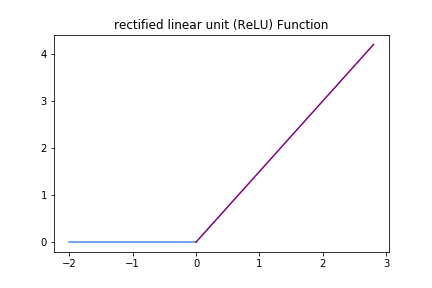
\includegraphics[width=0.4\textwidth]{fig/relu}
\end{figure}\begin{figure}[H]
	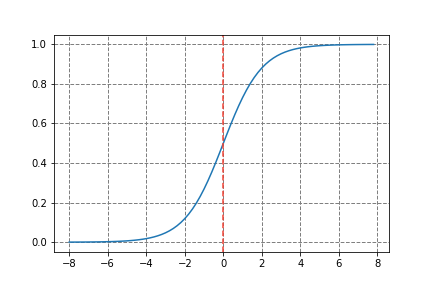
\includegraphics[width=0.4\textwidth]{fig/sigmoid}
\end{figure}}
\begin{python}
# Chapter 3 Pre-lecture Exercise
# 第三章课前练习
# @ Michael

# Import essential packages
# 导入必要扩展

import numpy as np
import matplotlib.pyplot as plt

# Play with colours in Python
# 简单的颜色绘图
# We will use matplotlib to plot a very simple function 
# with varied colours
# 我们将会使用 matplotlib 绘制简单的方程图形并且调试不同颜色

plt.plot([2], [3], 'bo')
plt.plot([4], [4], 'ro')
plt.plot([5], [2], 'go')
plt.axis([0, 6, 0, 7])  # change the range of axis
plt.grid(color='gray', linestyle='--', linewidth=1)  # add grid
plt.title('My first plot')


# plot ReLU function
x1 = np.arange(-2, 0.2, 0.2)
x2 = np.arange(0, 3, 0.2)
plt.plot(x1, 0*x1, color=(70/255, 136/255, 241/255))
# RGB(70, 136, 241)
plt.plot(x2, 1.5*x2, 'purple')
plt.title('rectified linear unit (ReLU) Function')


# plot sigmoid function
x3 = np.arange(-8, 8, 0.2)
y3 = np.exp(x3)/(1+np.exp(x3))
plt.plot(x3, y3)
plt.grid(color='gray', linestyle='--', linewidth=1)  # add grid
plt.axvline(x=0, color=(243/255, 66/255, 53/255), linestyle='--')
# add vertial line
\end{python}


\subsection{课堂讲义C2}



\subsection{课后练习C3}









\end{document}
